%----------------------------------------------------------------------------------------
%	SOLUTION 1
%----------------------------------------------------------------------------------------
\subsection*{Solution 1}
\paragraph{Summary:} The dataset has total $10$ attributes. One of them is sample ID number which is unique to each sample in most of the cases (though there are some duplicates). The other attributes are integer valued from $1$ to $10$. There are some missing values also for some samples. Therefore, the first step was to process the dataset.
\paragraph{Data processing:} I have replaced the missing values with the mode of the feature values of the samples with no missing values. More precisely, say $X_m$ and $X_f$ denote the the sets of samples with any missing values and no missing values respectively. Then, for sample $i$ with missing feature $m$,
\begin{align*}
	X_m[i, m] = \text{mode}(X_f[:, m]).
\end{align*}
Also, I have converted sample ID to categorical variable with two categories. The split point to divide the sample IDs into two categories are chosen to be the mean value of sample ID over all the samples. For other attributes, I tried both approaches with $10$ independent categories and two categories with split point chosen as $5$ (\textit{i.e.} attribute value $\leq\ 5$ denoted as $0$ and $1$ otherwise). I found that having two categories instead of $10$ gives better generalization accuracy and reduces variance. Therefore, I have converted all the attributes to categorical with two categories with split point chosen as the mean value of the range of the values of respective categories.

Majority vote has been chosen as the predicted label for a particular leaf node. Also, in case of sample ID, it is possible that a new test sample comes with completely new sample ID which has not been seen by the tree during training, therefore, having two categorical variables helps in this case which would have not been possible if we had different branches for different values of ID.
\paragraph{Calculation of weighted information gain:}In case of Adaboost, it is required to put different weights on samples while calculating the entropy. This can be done in two ways: (1) Calculating entropy based on weights of the samples instead of number of samples with different labels, (2) sample from training dataset with replacement according to the sample weights. I have tried both and found that, in case of approach (1), where the entropy of a particular leaf node is calculated by computing $entropy = -\frac{\sum_{i \in \mathcal{I}_p}D_i}{\sum_{i\in \mathcal{I}_p\cup\mathcal{I}_n}D_i}\log_2(\frac{\sum_{i \in \mathcal{I}_p}D_i}{\sum_{i\in \mathcal{I}_p\cup\mathcal{I}_n}D_i})-\frac{\sum_{i \in \mathcal{I}_n}D_i}{\sum_{i\in \mathcal{I}_p\cup\mathcal{I}_n}D_i}\log_2(\frac{\sum_{i \in \mathcal{I}_n}D_i}{\sum_{i\in \mathcal{I}_p\cup\mathcal{I}_n}D_i})$, where $\mathcal{I}_p, \mathcal{I}_n$ denote the set of indices of the positive and negative samples in the leaf node and $D_i$ denote the sample weight of sample $i$, it does not change if somehow Adaboost error hits $0.5$ error rate. Because, once Adaboost hits $0.5$ error rate, it does not change the weights of the samples in the successive iterations and therefore does not change the stumps thereafter. To avoid this, I have used sampling with replacements according to the sample weights and then fed the sampled train set to the stumps to learn. In this way we can have variations in the stump which helps in Adaboost learning.
\paragraph{Results:}Fig.~\ref{fig:q1_error_rate} shows the classification error rate as we increase the number of weak learners. It can be seen that, as the number of weak learners increases, the training error decreases. However, the test error decreases at first then freezes to decrease anymore and sometime increases also. This behavior denotes overtraining of the algorithm. Increasing the number of weak learners over-trains the algorithm and thus gives poor generalization. 
%%%%%%%%%%%%%%%%%%%%%%% ADABOOST ERROR %%%%%%%%%%%%%%%%%%%%%
\begin{figure}[!h]
	\centering
	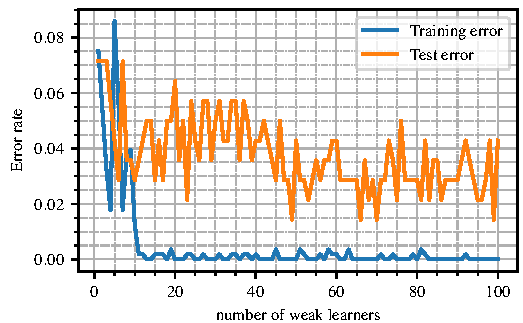
\includegraphics[scale=1.0,trim={0cm 0cm 0cm 0cm},clip]{./code/generatedPlots/q1_error_rate.pdf}
	\caption{Q1: Adaboost: Classification error rate on train and test sets}
	\label{fig:q1_error_rate}
\end{figure}